% -*- LaTeX -*-
% -*- coding: utf-8 -*-
%
% ~~~~~~~~~~~~~~~~~~~~~~~~~~~~~~~~~~~~~~~~~~~~~~~~~~~~~~~~~~~~~~~~~~~~~~~~~~~~~~
%
%                             michael a.g. aïvázis
%                      california institute of technology
%                      (c) 1998-2010  all rights reserved
%
% ~~~~~~~~~~~~~~~~~~~~~~~~~~~~~~~~~~~~~~~~~~~~~~~~~~~~~~~~~~~~~~~~~~~~~~~~~~~~~~
%

\lecture{Programming with MPI}{20100125}

% --------------------------------------
% template
\begin{frame}[fragile]
%
  \frametitle{Distributed memory parallelism}
%
  \begin{itemize}
%
  \item recall the generic layout of a distributed memory machine
%
    \begin{figure}
      \centering
      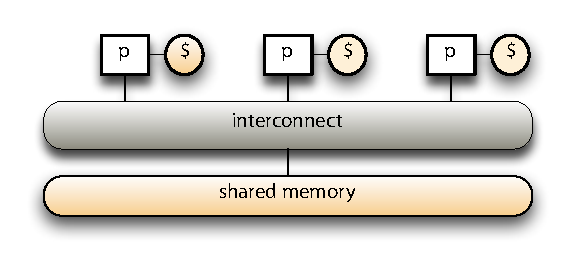
\includegraphics[scale=0.5]{figures/shared-memory.pdf}
    \end{figure}
    \vspace{-1.0em}
%
    \begin{itemize}
      \item each processor has its own private memory space
      \item processors communicate via the interconnect substrate
    \end{itemize}
%
  \item the programming model
    \begin{itemize}
    \item programs consist of a collection of $p$ named processes
    \item logically shared data must be partitioned among the processors
    \item communication and synchronization must be orchestrated explicitly 
    \end{itemize}
%
  \end{itemize}
%
\end{frame}

% end of file 
